%%%%%%%%%%%%%%%%%%%%%%%%%%%%%%
% LATEX-TEMPLATE TECHNISCH RAPPORT
%-------------------------------------------------------------------------------
% Voor informatie over het technisch rapport, zie
% http://practicumav.nl/onderzoeken/rapport.html
% Voor readme en meest recente versie van het template, zie
% https://gitlab-fnwi.uva.nl/informatica/LaTeX-template.git
%%%%%%%%%%%%%%%%%%%%%%%%%%%%%%

%-------------------------------------------------------------------------------
%	PACKAGES EN DOCUMENT CONFIGURATIE
%-------------------------------------------------------------------------------

\documentclass{uva-inf-article}
\usepackage[english]{babel}

\usepackage[
backend=biber,
style=numeric,
citestyle=numeric 
]{biblatex}

\usepackage{xcolor}
\usepackage{geometry}
\usepackage{amsmath}
\usepackage[linesnumbered,ruled]{algorithm2e}
\usepackage{color}
\usepackage{listings}
\usepackage{caption}

\newcounter{nalg}[section] % defines algorithm counter for chapter-level
\renewcommand{\thenalg}{\arabic{nalg}} %defines appearance of the algorithm counter
\DeclareCaptionLabelFormat{algocaption}{Algorithm \thenalg} % defines a new caption label as Algorithm x.y

\lstnewenvironment{pseudocode}[1][] %defines the algorithm listing environment
{   
    \refstepcounter{nalg} %increments algorithm number
    \captionsetup{labelformat=algocaption,labelsep=colon} %defines the caption setup for: it ises label format as the declared caption label above and makes label and caption text to be separated by a ':'
    \lstset{ %this is the stype
        breaklines=true,
        postbreak=\mbox{\textcolor{red}{$\hookrightarrow$}\space},
        mathescape=true,
        frame=tB,
        numbers=left, 
        numberstyle=\tiny,
        basicstyle=\scriptsize, 
        keywordstyle=\color{black}\bfseries\em,
        keywords={,input, output, return, for, function, in, if, else, foreach, while, begin, end, } %add the keywords you want, or load a language as Rubens explains in his comment above.
        numbers=left,
        xleftmargin=.04\textwidth,
        #1 % this is to add specific settings to an usage of this environment (for instnce, the caption and referable label)
    }
}
{}
\newcommand\todo[1]{\textcolor{red}{#1}}


\lstdefinestyle{mystyle}{
    basicstyle=\footnotesize,
    breakatwhitespace=false,         
    breaklines=true,                 
    captionpos=b,                    
    keepspaces=true,                 
    numbers=left,                    
    numbersep=5pt,                  
    showspaces=false,                
    showstringspaces=false,
    showtabs=false,                  
    tabsize=2,
    frame=single
}

\lstdefinestyle{pseudocodeStyle}{
    frame=single
}

\addbibresource{citations.bib}

%-------------------------------------------------------------------------------
%	GEGEVENS VOOR IN DE TITEL
%-------------------------------------------------------------------------------

% Vul de naam van de opdracht in.
\assignment{Software Evolution Series 2}
% Vul het soort opdracht in.
\assignmenttype{Report}
% Vul de titel van de eindopdracht in.
\title{Report}

% Vul de volledige namen van alle auteurs in.
\authors{Cornelius Ries; Piotr Kosytorz}
% Vul de corresponderende UvAnetID's in.
\uvanetids{11884827; 11876964}

% Vul altijd de naam in van diegene die het nakijkt, tutor of docent.
\tutor{}
% Vul eventueel ook de naam van de docent of vakcoordinator toe.
\docent{Riemer van Rozen}
% Vul hier de naam van de PAV-groep  in.
% \group{Group 7}
% Vul de naam van de cursus in.
\course{Software Evolution}
% Te vinden op onder andere Datanose.
\courseid{}

% Dit is de datum die op het document komt te staan. Standaard is dat vandaag.
\date{\today}

%-------------------------------------------------------------------------------
%	VOORPAGINA
%-------------------------------------------------------------------------------

\begin{document}
\maketitle

%-------------------------------------------------------------------------------
%	INHOUDSOPGAVE EN ABSTRACT
%-------------------------------------------------------------------------------

% Niet doen bij korte verslagen en rapporten
%\tableofcontents
%\begin{abstract}
%\lipsum[13]
%\end{abstract}

%-------------------------------------------------------------------------------
%	INTRODUCTIE
%-------------------------------------------------------------------------------

\section{Introduction}

This document presents our report for the "Series 2" assignment. To begin with, in chapter \ref{definitions}, we provide a few definitions to clarify some of the terms that are used in the reader and in this report. The next chapter focuses on the main algorithm of our clone detection as well as the approaches for detecting the different types of clones. Chapter 4 provides a description of our test suite. Chapter 5 focuses on the visual interface of the tool, explaining which requirements we chose and how we try to satisfy them with our visualizations. Chapter 6 serves as a manual for the tool, describing how to run and use it. The last chapter gives a conclusion on how the program works while analysing different projects and what could be improved.

\section{Definitions}\label{definitions}

In order to provide a tool to satisfy the assignment's objectives, a good understanding of the key concepts used in clone detection is needed. Based on a biref literature study, we have selected the following definitions as the base for our work and evaluation of the cloning problem:

\subsection{Clones and clone classes}

\begin{itemize}

	\item{\textbf{Clone relation} is an equivalence relation on code portions \cite{kamiya2002ccfinder}.}
	
	\item{\textbf{Clone pair} is a set of two code portions that are in clone relation with each other (compare \cite{kamiya2002ccfinder}).}
	
	\item{\textbf{Clone class} is an equivalence class of clone relation. In other words, it is a set of multiple (more than one) code portions which hold mutual clone relation to each other (compare \cite{kamiya2002ccfinder}).}
	
	\item{\textbf{The biggest clone} is is the biggest (has the largest number of lines of code) code portion, for which exists at least one code portion, which holds clone relation with it.}
	
	\item{\textbf{The biggest clone class} is the biggest equivalence class of clone relation (has the most elements) in the domain of examined project.}
	
\end{itemize}	

\subsection{Clone types}

\begin{itemize}

	\item{\textbf{Type-1 clones}
are per definition from \cite{koschke2008identifying} strict textual clones, excluding comments and white spaces.}

	\item{\textbf{Type-2 clones}
are per definition from \cite{koschke2008identifying}  \textit{a syntactically identical copy; only variable, type, or function identifiers have been changed}.}

	\item{\textbf{Type-3 clones}
are per definition from \cite{koschke2008identifying} copies with further changes like adding/removing statements.}

\end{itemize}

\section{Algorithm design}

\subsection{General algorithm design}

The idea and algorithm of our duplication detection is based on the
papers \cite{lazar2014clone} and \cite{baxter1998clone}. 
The main idea behind this approach is to use the abstract syntax tree for clone detection.
After creating the AST from the source files, the nodes are hashed into different buckets.
If a bucket has more than one element, it follows, that there are multiple locations in the source code of this node.
This counts as one clone class. 

For our implementation we decided to use the map feature of Rascal to represent the different buckets. The key of the map is the bucket and a relation of nodes to locations is the value. This approach allows use to easily select all matching nodes using the key.  We also only consider nodes that are bigger than a certain threshold. The size of a node is computed by simply counting all the sub-nodes of the node in question. The threshold is a parameter and can be specified when starting the clone detection.

There are also multiple types of clones that our tool can detect. These are type 1 and type 2 clones. The next two chapters explain the detection of type 1 and type 2 clones. Last but not least, we provide a short rationale, why we did not go for type 3 detection. We end this section by providing a textual representation of our main algorithm.

\subsection{Type-1 cleaning}\label{type1alg}

If using the AST approach, the bucket key is in general just the node itself. There was a change in the implementation of Rascal that shifted the \texttt{loc} (location of a node) and other informations of a node, from the annotations on the node, to information contained in the node. This leads to the problem, that matching of nodes or comparison between nodes is not possible anymore, because every location is unique. To circumvent the problem we remove the unnecessary information from all the relevant nodes. The actual cleaning \texttt{cleanNode} is done by visiting all the sub-nodes of a relevant node and replacing the node with a cleaned version of the original node using the \texttt{insert} statement.

\subsection{Type-2 cleaning}\label{type2alg}

For type 2 detection we also use the AST. To streamline all the information that is contained in the node we visit all the sub-nodes of a node,  and replace specific variables/identifiers/types with a general one. The replacement is done using the Rascal \texttt{visit - case => } notation.

\begin{lstlisting}[language=Java, style=mystyle,caption={Node elements stripping method for type-2 clone detection.},captionpos=b]
case Type _ => lang::java::m3::AST::float()
case Modifier _ => lang::java::m3::AST::\public()
case \method(_, _, a, b) => \method(lang::java::m3::AST::float(), "method", a, b)
case \method(_, _, a, b, c) => \method(lang::java::m3::AST::float(), "method", a, b, c)
case \parameter(a, _, b) => \parameter(a, "parameter", b)
case \vararg(a, _) => \vararg(a, "vararg") 
case \annotationTypeMember(a, _) => \annotationTypeMember(a, "annotationTypeMember")
case \annotationTypeMember(a, _, b) => \annotationTypeMember(a, "annotationTypeMember", b)
case \typeParameter(_, a) => \typeParameter("typeParameter", a)
case \constructor(_, a, b, c) => \constructor("constructor", a, b, c)
case \interface(_, a, b, c) => \interface("interface", a, b, c)
case \class(_, a, b, c) => \class("class", a, b, c)
case \enumConstant(_, a) => \enumConstant("enumConstant", a) 
case \enumConstant(_, a, b) => \enumConstant("enumConstant", a, b)
case \methodCall(a, _, b) => \methodCall(a, "methodCall", b)
case \methodCall(a, b, _, c) => \methodCall(a, b, "methodCall", c)
case \simpleName(_) => \simpleName("simpleName")
case \number(_) => \number("125681651")
case \variable(_, a) => \variable("variable", a) 
case \variable(_, a, b) => \variable("variable", a, b) 
case \booleanLiteral(_) => \booleanLiteral(true)
case \stringLiteral(_) => \stringLiteral("stringLiteral")
case \characterLiteral(_) => \characterLiteral("a")
\end{lstlisting}

\subsection{Type-3 approach}
While the tool does not detect type 3 clones, the basic idea behind type 3 detection is, that it should compute some sort of similarity between who nodes and consider it a duplication if the similarity is inside a specified threshold. The paper \cite{baxter1998clone} gives an idea on how to approach this. We tried to implement this, but it slowed down our clone detection by such a degree, that we decided to drop it and focus more on the visualizations and usability of the presentation. 

Also looking at the approach from \cite{baxter1998clone}, which relies on the size of node, it comes to question if using this approach is really sensible, because the size of a node does not really say anything about its contents. Two completely different nodes could be detected as clones, just because they share the same size.

In the next section we provide an exhaustive explanation of the applied algorithm and provide pseudocode for that. 

\subsection{The main algorithm}\label{main_alg}

In this section we provide a textual representation and explanation for our main algorithm. For further information please take a look into the source file \texttt{DuplicationsAnalyzer.rsc}.

\subsubsection{Consolidated general algorithm}

The main algorithm, as presented in the listing below, consists of four parts. In the first part, the algorithm generates a list of clone candidates based on the nodes previously obtained from the AST tree of the analysed project. The threshold, as mentioned earlier, is the number of sub nodes of an analysed node. After obtaining the clone candidates, the next step is to extract the true duplications from there. At this moment, the program doesn't have a list of clones yet, as it still has to filter out all the clones that are a part of a bigger clone (to stay with the biggest clone only). This happens in the next step (line 6). Finally, the obtained list would be shortly analysed and each found clone would be complemented with some metadata for presentation purposes. 

\begin{pseudocode}[caption={Consolidated general algorithm.}, label={alg0}]
 input: ast AST, int threshold
 output: set duplications
 begin
  mapOfCloneCandidates $\gets$ extractMapOfCloneCandidates(AST, threshold)
  setOfDuplications $\gets$ createAsetOfDuplications(mapOfCloneCandidates)
  filteredSetOfDuplications $\gets$ filterSetOfDuplications(setOfDuplications)
  duplications $\gets$ performFinalAnalyse(filteredSetOfDuplications)
  return duplications
 end       
\end{pseudocode}

\subsubsection{Extracting a map of clone candidates}

The first operation is to iterate through the whole AST tree (node by node) and to create a list (map) of all nodes that we want to investigate further. The main property of such a node is to match a minimal size threshold. In this case, size is determined by number of node's subnodes. 

The algorithms for methods \texttt{CleanNodeForType1Detection} and \texttt{CleanNodeForType2Detection} have been described respectively in sections \ref{type1alg} and \ref{type2alg}.

\begin{pseudocode}[caption={Extracting a map of clone candidates.}, label={alg1}]
 input: ast AST, int threshold
 output: map mapOfCandidates
 begin
  foreach (node in AST)
  begin
    if (size_of_node(node)  > threshold)
    begin
        node $\gets$ CleanNodeForType1Detection(node)
        node $\gets$ CleanNodeForType2Detection(node)
        mapOfCandidates $\gets$ mapOfCandidates + (node, metadata)
    end
  end
  return mapOfCandidates
 end       
\end{pseudocode}

\subsubsection{Creating a set of duplications}

Once the list of clones candidates is provided, it is time to compare them one by one.

\begin{pseudocode}[caption={Creating a set of duplications.}, label={alg2}]
 input: map mapOfCandidates
 output: set setOfDuplications
 begin
  foreach (key in mapOfCandidates)
  begin
    tempListOfDuplications $\gets$ mapOfCandidates[key]
    if (size of tempListOfDuplications > 1)
    begin
        setOfDuplications $\gets$ setOfDuplications + tempListOfDuplications
    end
  end
  return setOfDuplications
 end       
\end{pseudocode}

\subsubsection{Filtering the set of duplications}

To filter all clone classes that are already fully contained in another clone class we basically
use a for loop in a for loop. This combination checks if there is another clone class whose locations contain all the locations as the current clone class. If there is none, the current clone class is added to a new set of filtered clone classes.
In the actual code this is achieved by using a reducer combined with any and all clauses in the condition statement.

\begin{pseudocode}[caption={Filtering the set of duplications.}, label={alg3}]
input: set setOfDuplications
output: set filteredSetOfDuplications
begin
  foreach (duplicationLocations in setOfDuplications)
    begin
      if (not any(duplicationLocations2 in setOfDuplications contains duplicationLocations)
      begin
        filteredSetOfDuplications  $\gets$ filteredSetOfDuplications + duplicationLocations
      end
    end
  return filteredSetOfDuplications
end
\end{pseudocode}

\subsubsection{Final analyse and enriching with metadata}

The last algorithm collects the filtered clone classes in the output data structure.
The data structure contains the locations and the clone type. 

\begin{pseudocode}[caption={Final analyse and enriching with metadata.}, label={alg4}]
 input: set filteredSetOfDuplications
 output: set duplications
 begin
   foreach (duplication in filteredSetOfDuplications)
    locations $\gets$ duplication.locations
    cloneType $\gets$ CleanNodeForType1Detection(locations[0]) == CleanNodeForType1Detection(locations[1]) ? 1 : 2
    duplications $\gets$ Duplication(locations, cloneType)
   end
  return duplications
 end       
\end{pseudocode}

\section{Main program validity}

We provide an automatic testing suite to verify that the tool works as designed. To maintain a good separation of concerns between implementation and tests, all tests are in separate files that extend their original Rascal module. This will result in better maintainability, readability and extensibility for the future. 

The tests are split in random generated tests where applicable. For example while operating on files and their locations, Rascal is not able to provide a proper generator for reading the contents of a file. For this we provide three test files that are used in tests where files are needed. 

Especially the Clone Detection is covered with random test generators, testing the properties of the tested functions as well as tests where the implementation is tested against the provided test files to assure the continued working in case of refactoring. For design changes the tests may have to be adjusted.

To run the tests, import all the modules below and execute \texttt{:test} in the Rascal console. The \texttt{projectLocation} in \texttt{Configuration.rsc} has to be set to the projects location in your eclipse workspace!

\begin{itemize}

\item
  DuplicationsAnalyzerTests
\item
  RaterTests
\item
  UtilsTests
\item
  VolumeAnalyzerTests
\end{itemize}


\section{The tool}

\subsection{Introduction}
As it is stated in the assignment, we were supposed to provide a tool for clone detection that we actually would use ourselves.  Since web technologies provide currently the best tools to present data and are easy to implement, and since there is a web server in Rascal, we have decided to provide a JavaScript application as the user interface for our tool. 

The front-end application is served directly from our Rascal application, which means that no extra configuration is required to use it with the provided clone detector. It is written in ReactJS \footnote{Facebook Inc. 2017. React. [ONLINE] Available at: \url{https://reactjs.org/}. [Accessed 14 December 2017].
}. The main (Rascal) application provides a number of REST API endpoints that the JavaScript application uses to obtain data and request a project analysis. 

\subsection{Requirements}
The main requirements from the perspective of code maintainer that we wanted to address with our tool are the following: 

\begin{itemize}
    \item{To get a comprehensible overview (of code quality and duplications)}
    \item{To get insight into the clones and navigate effortlessly through elements}
    \item{See how the clones are shared among files in the project (to improve comprehension ) }
\end{itemize}

The following paragraphs describe how the tool that we've created satisfies the stated requirements. 

\subsubsection{Comprehensible overview}
The first portion of information that a maintainer receives after running a code analysis should be comprehensive and valuable. For this matter we have decided to extend the overview of code quality factors from series 1 (the general statistics and SIG rating table) and provide an additional overview of clones statistics, that contains the following metrics: 
\begin{itemize}
	\item{Number of clones}
	\item{Number of clone classes}
	\item{Biggest clone and its location}
	\item{Biggest clone class and its location}
\end{itemize}

\subsubsection{Insight and effortless navigation}
As it is well explained in Baxter et al., reduction of the maintainer's cognitive overhead is one of the main branches of Cognitive Design Elements for Software Exploration \cite{baxter1998clone}. We provide therefore a searchable data table that contains clone classes and containing files with some extra metadata, like clone type, number of lines per clone and number of files per clone class. All fields in the table are searchable, and after clicking on a certain row, the tool presents clone details in a pop-up window. 

We consider the data table to be actually the most handy and practical tool a software maintainer might desire. Even though its simplicity, it is an extremely flexible tool that allows the user to get all available details of a clone detection result.

\subsubsection{Insight into clones sharing among project's files}
This last requirement refers to clone location among different files in the project. This requirement could be satisfied only with a suitable visualization. We have decided to use a force directed graph\footnote{\url{https://en.wikipedia.org/wiki/Force-directed_graph_drawing}} and an arc graph diagram \footnote{\url{https://en.wikipedia.org/wiki/Arc_diagram}} for this purpose. 

\paragraph{Force graph}
In our implementation we have used a React Component provided by Uber\footnote{\url{https://github.com/uber/react-vis-force}}, which after some modifications made a perfect solution to our needs. 

In our solution, each node (dot) represents a single file in the project, which contains at least one clone. Each line between two nodes represents a shared clone. The Color of each node represents the number of related files - the darker, the more nodes. A legend provided in our tool explains in detail the meaning of each color. 

In the visualization, files with only internal clones are represented as single dots with no relations to other files. Files that share one or more clones form subgraphs. The very nice property of a force directed graph is, that the elements with the most relations to each other are being attracted to each other. They form subgraphs. On the other hand, the subgraphs repel each other, what makes a visual effect of multiple separate constellations of items that share common value (in our case - clones). 

Our approach to visualization made it possible to quickly and easily determine groups of files that share clones, and have partially probably similar purpose in the project. Such groups of files are clearly refactoring candidates. 

The tool provides also an extremely handy details preview for files in this visualization. After clicking on a single node (representing a file), the tool will show file details with all clones identified in this file, a list files that share clone classes with this file, and clone details per each related file. 

\paragraph{Arc diagram}
We got the initial idea for this diagram from the bibwiz\
{\url{http://bibviz.com/}} project. This project shows bible contradictions among the different books in the bible as an arc diagram. After studying the source code, we adapted the main javascript code (which uses d3 to draw the diagram) for our needs.

The arc diagram is a nice way to get more information about the clone distribution in a project. While the force graph only shows the cloned files, the arc diagram shows all the files in the project as blue bars. The length of the bar further indicated the file's length (line count). The arcs in the diagram represent all the different clone classes that exist in the project. By hovering over a bar or arc, either the current file or all the files in the selected clone class are displayed.

One weakness of this diagram is, that clones in a single file are not visible. This is where the force graph comes in handy. This is also why we decided to use both diagrams in our solution, because they complement each other.

\section{Tool manual}

\subsection{Installation}

The Rascal clone detector is provided with a built of our visualization tool. Source code for that part of the project is available at: \url{https://github.com/piotrkosytorz/software-evolution/tree/master/piotr.kosytorz/series1/src}. The source code for the visualization part can be found at \url{https://github.com/piotrkosytorz/software-evolution/tree/master/piotr.kosytorz/series1/visualization}.

If you prefer to use \texttt{git}, you can clone the whole project in your console with:

\begin{verbatim}
git clone https://github.com/piotrkosytorz/software-evolution.git
\end{verbatim}

The Rascal source code is in \texttt{piotr.kosytorz/series1/src/src}.

\subsection{Program setup}

In order to run the program, please follow the steps:

\begin{enumerate}
\item Please import the Rascal part as a project into your eclipse with a working Rascal installation.
\item
  Open \texttt{Configuration.rsc} and adjust the location of the \texttt{projectLocation} to match the path of the project to your eclise workspace.
\item Do the same for the \texttt{smallSqlProject} and \texttt{hqSqlProject}.
\item Start a Rascal console and import the \texttt{Main} module.
\item Run \texttt{startServe();}
\item Open a browser and point it towards \url{http://localhost:5433/index.hmtl}.
\end{enumerate}

\subsection{How to use}

The application opens in a web browser as a web application. Figure \ref{screenshot1} (Appendix A in \ref{appendix:a}) presents the initial view of the application. Figures \ref{screenshot2}-\ref{screenshot3}-\ref{screenshot4} give example views of the visualizations.

\begin{itemize}

\item{In the top left corner (box marked with \textbf{1}) of the view, a form is placed. From the dropdown list on the left side the user can select one of the pre configured projects, and in the field that's located next to it, he may adjust the unit size threshold for the clone detector. Clicking on the \textbf{Run analyser} button will start the detector. After the analysis is finished, the status changes. Since that moment all data generated by the code detector is available in the visualization tool for further investigation. }

\item{On the left side (box marked with \textbf{2}), a menu with available tools is located. }
\item{The rest of the view (box marked with \textbf{3}) presents the chosen tools. }
\item{The box marked with \textbf{4} shows an example view of the data-table visualization. One row equals one clone class. By clicking on the row a modal dialog appears with more information about the clone class.}
\item{The box marked with \textbf{5} shows an example view of the constellation visualization. The legend on the right explains how to read it. By clicking on a dot (file) a modal dialog opens with all the clone classes of that file. }
\item{The box marked with \textbf{6} shows an example view of the project distribution visualization. The legend on the right explains how to read it. By hovering over a bar or arc the relevant information is displayed.}
\end{itemize}

\section{Summary}
Our aim in this assignment was to provide a clone detector and a tool to analyse those clones, that we would use ourselves. We believe that we have succeeded. 

We decided to apply a different approach than setting the minimum of 6 lines of a clone class, because of several reasons. The first being, that like this you can fine tune for your project how big a clone should be. Of course the threshold could have been set up as lines as well, but this would have meant that for example getters and setters would have been detected as clones. This leads us to the next reason for our decision. With the node size a getter/setter is not detected, but complex on line statements, that should be put into reusable constants are detected as clones. The last reason is, that there was no evidence put forth in the papers why they used the 6 line minimum.

We also see some further room for improvement. Obviously type 3 detection would be one thing to integrate into our solution. But there is also the possibility for storing the analysis into some sort of data storage for caching. At the moment, if the application is stopped, all results are lost. The last thing that could be built on top of that would be a incremental analysis using the already stored data. Some sort of mechanism (like last modified date for file) could be used to skip previously processed files.

Our solution works very well with medium and small projects like \texttt{smallSQL}, where the analyse time oscillates around 1 minute and 30 seconds, depending on the size of the threshold. For big project, like \texttt{hsqldb}, the execution time runs up to 29 minutes. The detailed data table in our visualization tool works also perfectly with that project, however the visualization on the force graph is not that transparent any more, due to a huge number of files that won't fit one one screen. Another approach where the user/maintainer would be able to filter the files beforehand, would probably solve the problem. 

In the end, we are happy with our outcomes. 

%-------------------------------------------------------------------------------
%	REFERENTIES
%-------------------------------------------------------------------------------

\printbibliography

%-------------------------------------------------------------------------------
%	BIJLAGEN EN EINDE
%-------------------------------------------------------------------------------

\section{Appendix A: Screenshots}\label{appendix:a}

\begin{figure}[!htb]
	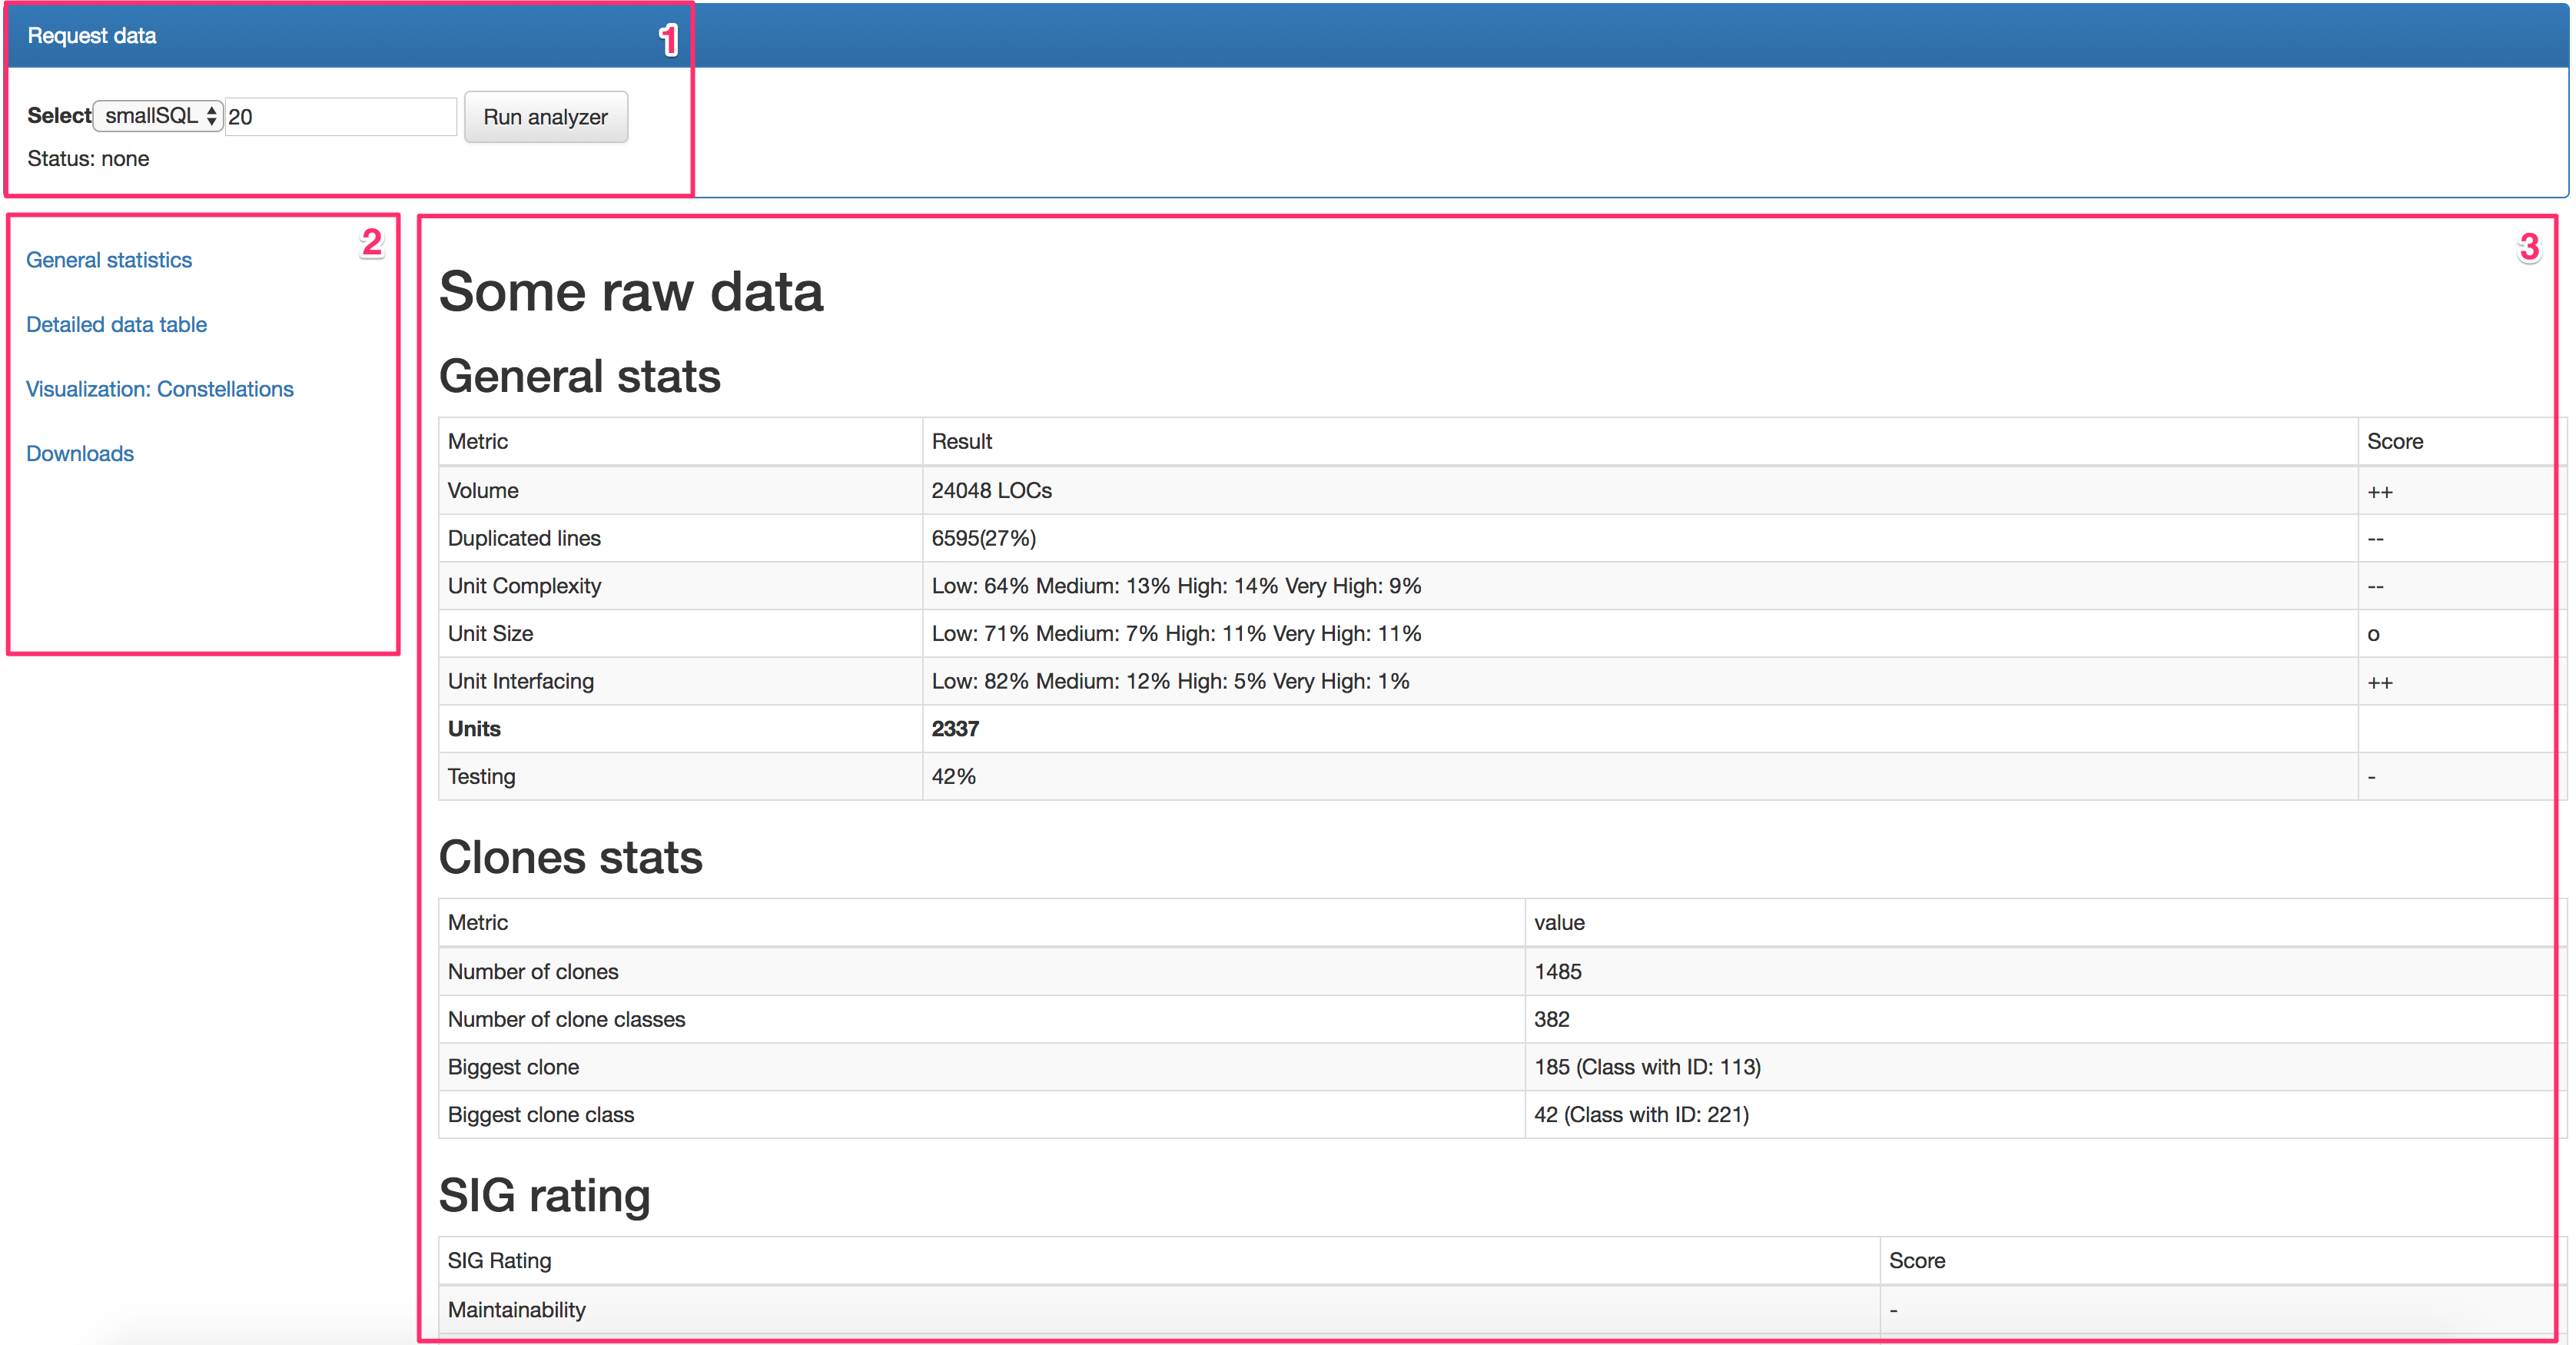
\includegraphics[width=\textwidth]{visualization1}
	\centering
	\caption{Clone detection tool screenshot.}
	\label{screenshot1}
\end{figure}

\begin{figure}[!htb]
	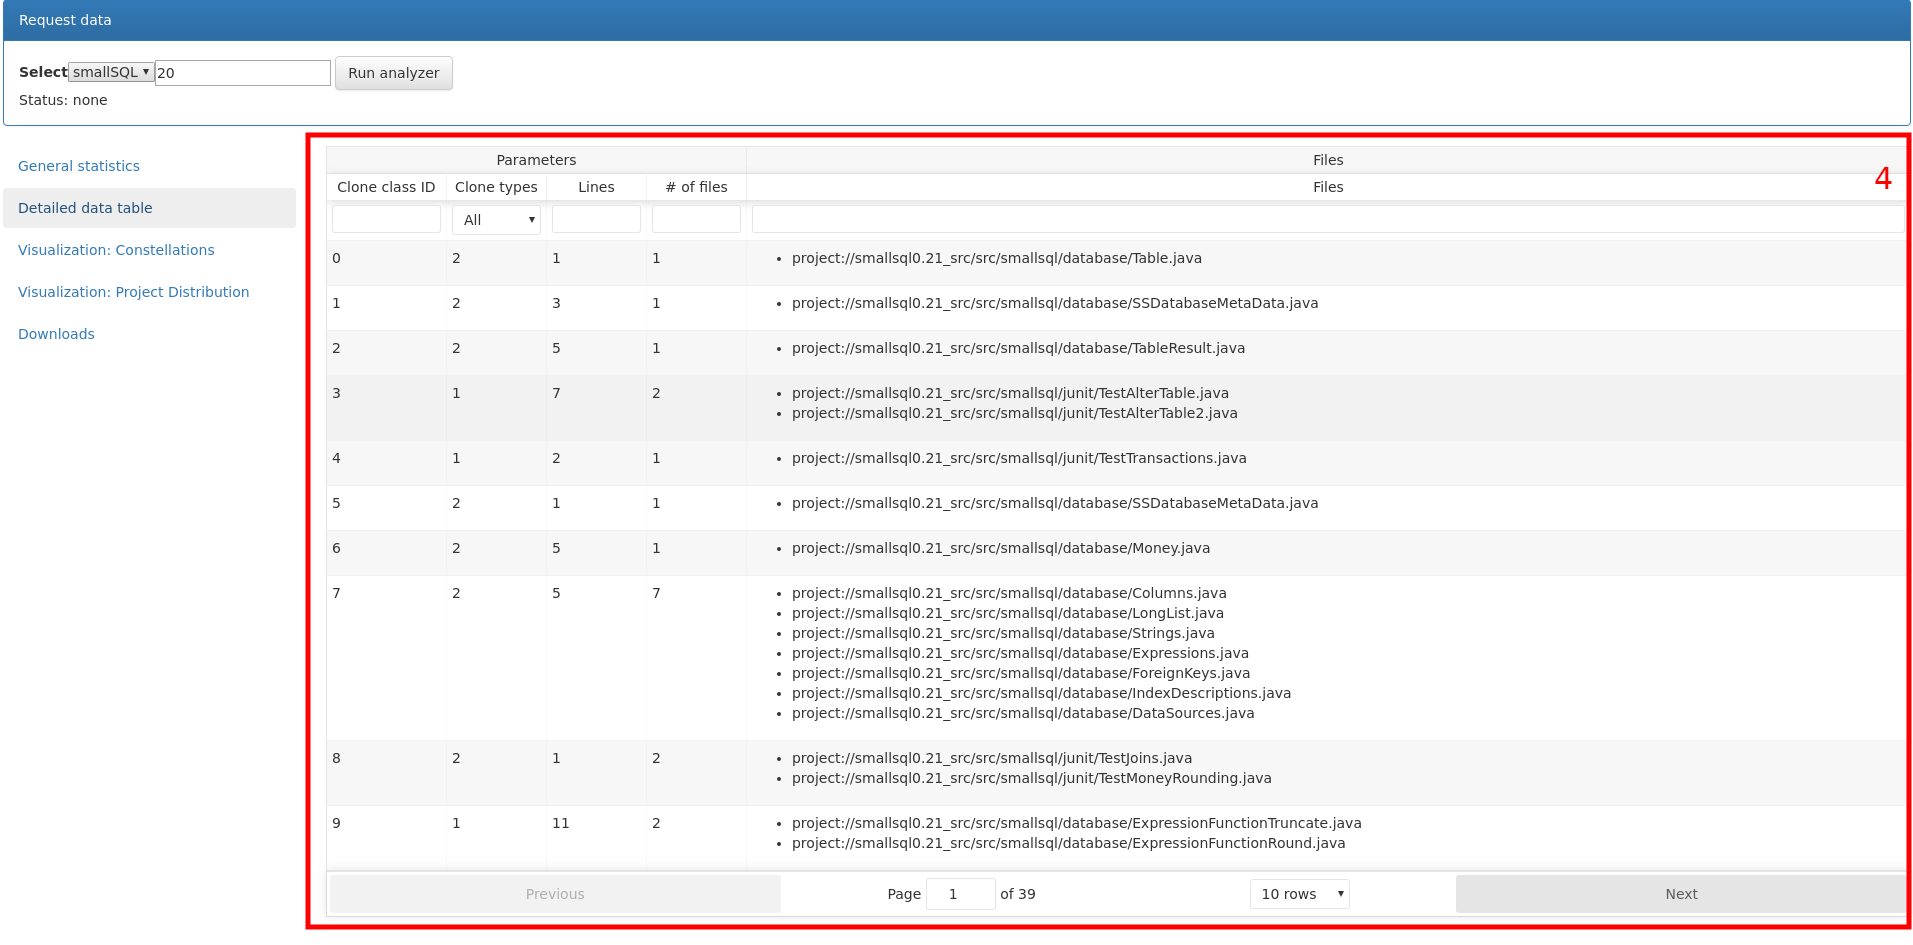
\includegraphics[width=\textwidth]{visualization2}
	\centering
	\caption{Data table overview screenshot.}
	\label{screenshot2}
\end{figure}

\begin{figure}[!htb]
	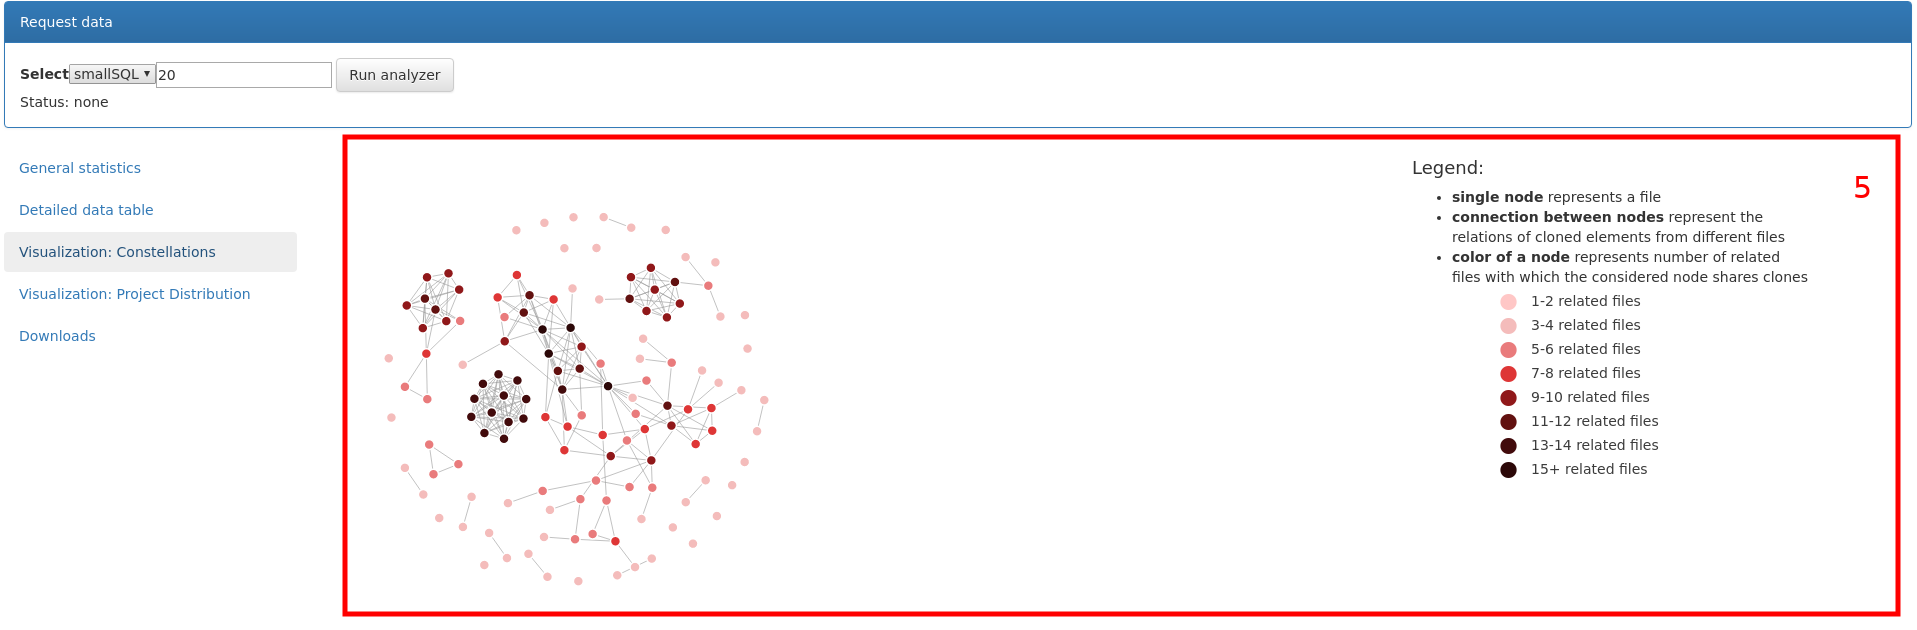
\includegraphics[width=\textwidth]{visualization3}
	\centering
	\caption{Constellations screenshot.}
	\label{screenshot3}
\end{figure}

\begin{figure}[!htb]
	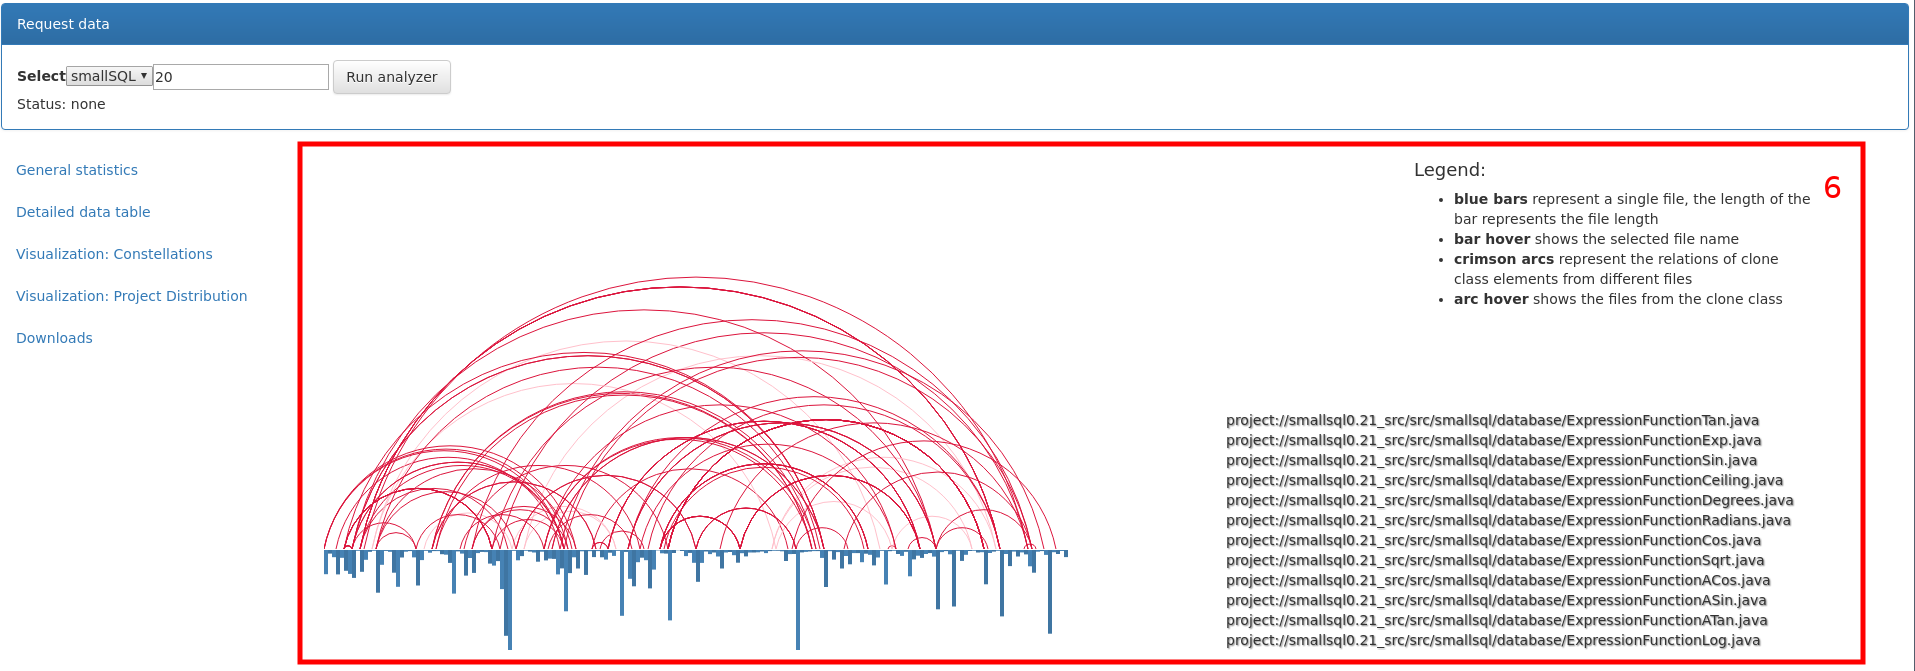
\includegraphics[width=\textwidth]{visualization4}
	\centering
	\caption{Project distribution screenshot.}
	\label{screenshot4}
\end{figure}

%\section{Bijlage B}
%\section{Bijlage C}
\end{document}
